%! TEX root = ../main.tex
\documentclass[main]{subfiles}

\begin{document}
\silentchapter{\texorpdfstring
{$\sqrt{\quad}\rightarrow$  基本的には外す}
{√→基本的には外す}}

\begin{newmondai}{例題}{2}{今週の積分}{**}
    \int_0^{2\pi} \sqrt{1+\cos x} dx
\end{newmondai}

\approachitem{$\sqrt{\quad}\rightarrow$  基本的には外す}

\solutionhead
\hfill
以下に計算手順を示す.
\hfill\
\begin{equation*}
    \sqrt{1+\cos x} = \sqrt{2\cos ^2 \frac{x}{2}} = \sqrt{2}\left| \cos \frac{x}{2} \right| = 
    \begin{cases}
        \sqrt{2} \cos \frac{x}{2} \qquad (0\leqq x \leqq \pi)\\
        -\sqrt{2} \cos \frac{x}{2} \qquad (\pi\leqq x \leqq 2\pi)
    \end{cases}
\end{equation*}
よって、
\begin{align*}
    \int ^{2\pi}_0 \sqrt{1+\cos x} dx
        &= \int^\pi_0 \sqrt{2} \cos \frac{x}{2}dx + \int^{2\pi}_\pi \left(-\sqrt{2} \cos \frac{x}{2}\right)dx \\
        &= \sqrt{2} \left\{\int^\pi_0 \cos \frac{x}{2}dx - \int^{2\pi}_\pi \cos \frac{x}{2}dx \right\} \\
        &= \sqrt{2} \left\{ \left[ 2\sin \frac{x}{2} \right]^\pi_0 - \left[ 2\sin \frac{x}{2} \right]^{2\pi}_\pi \right\} \\
        &= \sqrt{2} \left\{ (2-0) - (0-2) \right\} \\
        &= \boldsymbol{4 \sqrt{2}}
\end{align*}
\begin{figure}[H]
    \centering
    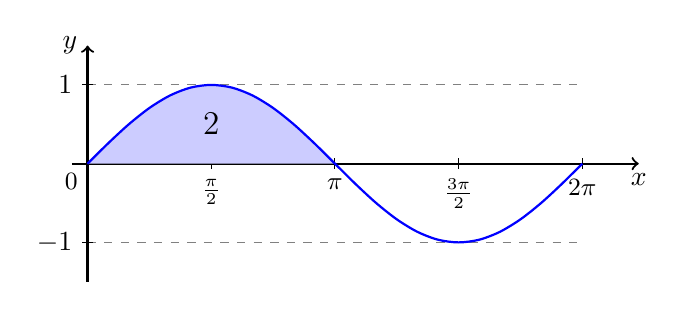
\begin{tikzpicture}
        % --- 座標軸の描画 ---
        % x軸 (矢印付き)
        \draw[->, thick] (-0.2,0) -- (7,0) node[below] {$x$};
        % y軸 (矢印付き)
        \draw[->, thick] (0,-1.5) -- (0,1.5) node[left] {$y$};

        % --- グリッド線の描画 ---
        \draw[gray, thin, dashed] (0,1) -- (6.28,1);
        \draw[gray, thin, dashed] (0,-1) -- (6.28,-1);

        % --- 目盛りの描画 ---
        % x軸の目盛りとラベル
        % \foreach <変数>/<ラベル> in {<値1>/<ラベル1>, <値2>/<ラベル2>, ...}
        \foreach \x/\label in {1.5708/\frac{\pi}{2}, 3.14159/\pi, 4.71238/\frac{3\pi}{2}, 6.28318/2\pi} {
            \draw (\x, 2pt) -- (\x, -2pt) node[below, font=\small] {$\label$};
        }
        \node[below left, font=\small] at (0,0) {$0$}; % 原点のラベル

        % y軸の目盛りとラベル
        \foreach \y in {-1, 1} {
            \draw (2pt, \y) -- (-2pt, \y) node[left] {$\y$};
        }

        % ★★★ 1. 0からπまでの領域を塗りつぶす ★★★
        % グラフの線を描く前に塗りつぶしを行う
        \fill[blue!20] (0,0) -- plot[domain=0:pi, smooth, variable=\x] ({\x}, {sin(\x r)}) -- (pi,0) -- cycle;

        % --- 正弦波のプロット ---
        % 【重要】TikZのsin()は角度(度)を引数に取るため、
        % ラジアンの変数 \x の後ろに 'r' を付けて度に変換します。
        \draw[
            domain=0:2*pi,      % 定義域 (0から2πまで)
            smooth,             % 滑らかな線で描画
            variable=\x,        % 変数を\xとする
            blue,               % 色を青に
            thick               % 太い線で
        ] plot ({\x}, {sin(\x r)});

        % ★★★ 2. 塗りつぶした領域にテキストを描画 ★★★
        % 座標 (π/2, 0.7) あたりにノードを配置
        \node[font=\large] at (1.57, 0.5) {$2$};

    \end{tikzpicture}
    \caption{$y=\sin x$ のグラフ ($0 \le x \le 2\pi$)}
    \label{fig:sine_wave_tikz}
\end{figure}

\begin{figure}[H]
    \centering
    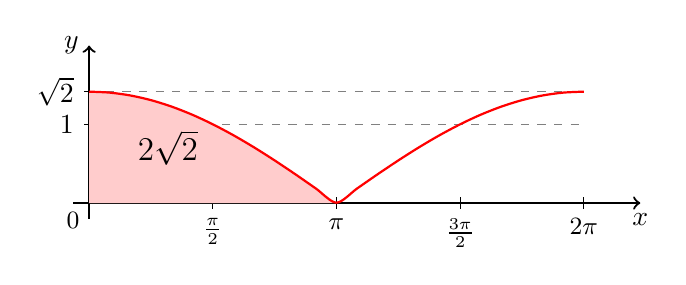
\begin{tikzpicture}
        % --- 座標軸 ---
        \draw[->, thick] (-0.2,0) -- (7,0) node[below] {$x$};
        \draw[->, thick] (0,-0.2) -- (0,2) node[left] {$y$};

        % --- グリッド線 ---
        \draw[gray, thin, dashed] (0,1) -- (6.28,1);
        \draw[gray, thin, dashed] (0,1.414) -- (6.28,1.414);

        % --- 目盛り ---
        % x軸
        \foreach \x/\label in {1.5708/\frac{\pi}{2}, 3.14159/\pi, 4.71238/\frac{3\pi}{2}, 6.28318/2\pi} {
            \draw (\x, 2pt) -- (\x, -2pt) node[below, font=\small] {$\label$};
        }
        \node[below left, font=\small] at (0,0) {$0$};
        % y軸
        \draw (2pt, 1) -- (-2pt, 1) node[left] {$1$};
        \draw (2pt, 1.414) -- (-2pt, 1.414) node[left] {$\sqrt{2}$};

        % ★★★ 1. 0からπまでの領域を塗りつぶす ★★★
        % グラフの線を描く前に塗りつぶしを行う
        \fill[red!20] (0,0) -- plot[domain=0:pi, smooth, variable=\x] ({\x}, {sqrt(1+cos(\x r))}) -- (pi,0) -- cycle;

        % --- グラフのプロット ---
        % 【重要】cos()も度数法のため、ラジアンの \x に 'r' をつけて変換
        \draw[
            domain=0:2*pi,
            smooth,
            variable=\x,
            red,
            thick
        ] plot ({\x}, {sqrt(1+cos(\x r))});

        % ★★★ 2. 塗りつぶした領域にテキストを描画 ★★★
        % 座標 (π/2, 0.7) あたりにノードを配置
        \node[font=\large] at (1, 0.7) {$2\sqrt{2}$};

    \end{tikzpicture}
    \caption{$y=\sqrt{1+\cos x}$ のグラフ ($0 \le x \le 2\pi$)}
    \label{fig:sqrt_cos_tikz}
\end{figure}

\end{document}